
%\documentclass{article}
\documentclass{vldb}
%\documentclass[10pt,conference]{IEEEtran}
%\documentclass{sig-alternate}
%\usepackage[utf8]{inputenc}
%\usepackage{algorithm2e}
%\usepackage[noend]{algorithm2e}
%\usepackage[boxed,commentsnumbered]{algorithm2e}
\usepackage{algorithmic}
\usepackage{algorithm}
%\usepackage{algorithmicx}
\usepackage{listings}
\usepackage{color}
\usepackage{xspace}
\usepackage{graphicx}
\usepackage{caption}
\DeclareCaptionType{copyrightbox} % Temporary hack to use the caption package
\usepackage{subcaption}
\usepackage{alltt}
\usepackage{balance}
\usepackage{hyperref}
\usepackage{paralist}
%\usepackage[top=0.75in, bottom=1in, left = 0.68in, right=0.68in]{geometry}
\usepackage{cite}
\usepackage{amsmath}


\newcommand{\ceg}[1]{{\textcolor{green}{#1 --- CEG}}}
\newcommand{\dzw}[1]{{\textcolor{magenta}{#1 --- CEG}}}
\newcommand{\eat}[1]{}
\newcommand{\qgram}{$q$-gram\xspace}
\definecolor{gray}{rgb}{0.5,0.5,0.5}
\newcommand{\added}[1]{\textcolor{blue}{#1}}
\newcommand{\changed}[1]{\textcolor{red}{#1}}
\newcommand{\removed}[1]{\textcolor{gray}{#1}}


\definecolor{light-gray}{gray}{0.15}
\newcommand{\thereviewer}[1]{\textcolor{light-gray}{\textit{#1}}}

\newcommand{\hide}[2]{#2}

\newenvironment{compactitemize}%
    {\begin{list}{}{
       \renewcommand{\makelabel}[1]{\bf $\bullet$}\hfil%
       \settowidth{\labelwidth}{\bf $\bullet$}%
       \setlength{\partopsep}{0mm}%
       \setlength{\parsep}{0mm}%
       \setlength{\parindent}{0mm}%
       \setlength{\itemsep}{0mm}%
       \setlength{\topsep}{0mm}%
       \setlength{\leftmargin}{\labelwidth}%
       \addtolength{\leftmargin}{\labelsep}
     }}%
    {\end{list}}

% Try to get rid of orphans
%\clubpenalty=10000
%\widowpenalty = 10000

\title{Entity Compression for Incremental Entity Resolution}

\numberofauthors{2}
\author{\alignauthor{Christan Earl Grant}\\
    \affaddr{University of Florida}\\
    \affaddr{Dept.\ of Computer Science}\\
    \affaddr{Gainesville, Florida, USA} \\
    \email{cgrant@cise.ufl.edu}\\
\alignauthor{Daisy Zhe Wang}\\
    \affaddr{University of Florida}\\
    \affaddr{Dept.\ of Computer Science}\\
    \affaddr{Gainesville, Florida, USA}\\
    \email{daisyw@cise.ufl.edu}\\
}

\begin{document}
\maketitle



\begin{abstract}
%\small\baselineskip=9pt
Increasingly, organizations have employed methods to understand unstructured text across the web.
Entity resolution is used to identify mentions in large, streaming text corpora.
Sampling-based entity resolution using Markov Chain Monte Carlo (MCMC) techniques guarantees convergence to a stationary distribution and can jump out of local optimum.
When performing entity resolution over streams of incoming data, the growing quantity of data amplifies two main issues.
First, because the sampling process is random, many iterations are wasted attempting to resolve unambiguous entities.
Second, the quadratic runtime for scoring entities becomes prohibitive for largest entities.
%When new documents are continuously updated the above issues are exacerbated.
Frequent streaming updates from the web exacerbate these difficulties.
In this paper, we discuss the creation of a proposal optimizer, in the spirit of database optimizers.
This optimizer observes the proposal updates to the entity resolution model
then makes recommendations to improve the processing and storage of the model.
We motivate the use of compression techniques to reduce the amount of processing when scoring MCMC updates proposal.
We also discuss statistical early-stopping techniques for scoring entities.
We describe our initial progress over a large entity resolution data set and
how an optimizer can improve performance when processing entity resolution streams.


\end{abstract}



\section{Introduction}

% What is the problem
The storage of user generated content within systems has introduced 
vast amounts of data.
To correctly process this data must be cleaned. 
Entity resolution is an important part of the ubiquitous cleaning task.
Entity Resolution (ER) is the problem of resolving records in
a data set that correspond the same real world entity.

% Why is the problem hard
Entity resolution is a notoriously computationally difficult problem.
Several efforts in different domains have made outstanding progress~\cite{}.
The main issues still affecting runtimes of ER systems are
twofold, first, the computation of large entities and second, excessive
computation spent resolving unambiguous entities.
Optimization that touches these critical portions is wholly understudied.
We argue that compression and approximation 
techniques can efficiently decrease the runtimes of traditional ER systems.

There is not one size fits all techniques even inside sampling algorithms~\cite{sculley2006compression}.

% What are the technical challenges and validation
Some recently, researchers have suggest methods of compressing entities.
Wick et al Heirchical \ldots

Singh et all efficient factoring % http://people.cs.umass.edu/~sameer/files/mcmcmc-emnlp12-ppt.pdf

Each of these methods has drawbacks \ldots

% How we differ
In this paper, we train a multi-class classifier to optimize the decision of
the sampling inference technique to apply.


% Our contributions
We make the following contributions

\begin{itemize}
\item We identify several techniques to speed up sampling past the baseline~\ref{}.
\item We create an optimizer to choose parameters and methods at run time~\ref{}.
\item We empirically evaluate these methods over a large data set~\ref{}.
\end{itemize}



% Links to people who used vectorization
% http://citusdata.github.io/cstore_fdw/
% http://www.drdobbs.com/parallel/parallel-in-place-merge-sort/240169094?pgno=2



\section{Background}

Entity Resolution

Blocking

The distribution of entitiy sizes


\section{Related Work}

Wick et al

Sameer Singh

Pay as you go ER



\section{Problem Statement}

We have two problems.
First,
Given an Entity $\mathcal{E}$ how can we create a
a structure with minimal total size.
Second, How can we incrementally add and remove items 
from the compressed structure.
Third, how can we iterate over or sample from the
compressed data structure to perform uncompression.




Show Distribution of Entity sizes in the data set

We can take advantage of the redundancy within
large entities and compress the entities.

We look to perform add, remove and iterate operations
over the compressed entity sets.  






\section{Algorithms}



\section{Implementation}

In this section we first present a microbenchmark to validate our invsitgation of entity approximation and compression.
We then discuss the implementation of the compression and approximation techniques over a large real-world
cross-document coreference corpus.

\subsection{Microbenchmark}
\label{sec:microbenchmark}
To increase our intuition of early stopping techniques we simulated the MCMC proposal processes. 
We hypothesis that there was bould a clear range values where performing the
baseline cluster sampling would be faster when compared to early stopping methods.
We arrange entity clusters of increasing time and we compute the time (in clock ticks)
each proposal takes to compute the arrangement of the clusters.
The data in the clusters are disctributed uniformly and for this experiment each cluster point
was 5 dimensional.
For the baseline cluster score computation we used a pairwise calculated of the average cosine distance
with and without the mention.
To compute early stopping we set a confidence threshold to $0.8$ and the early
stopping code stopped computation when the error predition was under $20\%$.
There was no difference in the proposal choices between the baseline and the early sorting method. 

The simulations were developped in \texttt{GNU C++11} and compiled with \texttt{g++ -O3}. 
The CPU was an 8 core intel i7 with 3.2 HGz and 12 GBs of Memory.
Each arrangement was run 5 times and results averages.


Experiment Results\ldots
The result of this experiment is summarized in Figure~\ref{fig:clustering-v-early-stopping}.
On the x-axis is the number of mentions in the source and destination clusteris for each proposal. 
The y-axsis is the number of clock ticks on a log scale.

\begin{figure}
\centering
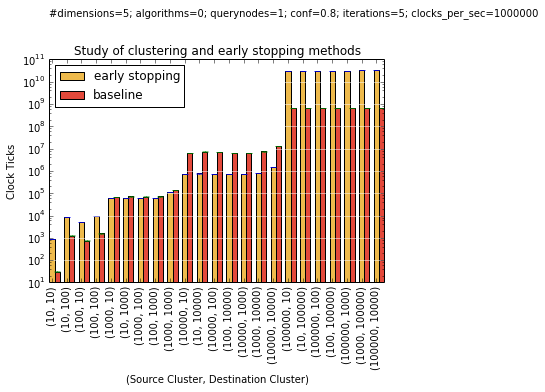
\includegraphics[width=\columnwidth, clip=true,trim=0cm 0cm 0cm 1cm]{media/clustering-v-early-stopping.png}
\caption{Comparison of baseline verses early stopping methods.}
\label{fig:clustering-v-early-stopping}
\end{figure}

We observe that for proposals with less than 100 and 1000 source and
destination mentions, the performance of the baseline proposer is better than
or almost equal to that of the more sorted early stopping method.
For proposals that contain an entity cluster with more than 10000 mentions
the early stopping method performs significantly better than the baseline method.

The optimization found in predictable code paths make simple implementations
like the baseline method attactive for small cluster sizes.
In addtion, $82\%$ of the entities in the truthed Wiki-Links data sets are less
that 1000 mentions in size and $45\%$ of the entities contain less than 100
mentions.

The results of the microbenchmark suggests that different proposal estimation techniques are useful at different times.




\subsection{Wiki Link Corpus}




\section{Evaluation}
%% TODO change to Discussion?





\section{Summary}

In this paper, we describe an initial approach for optimizing sampling for the entity resolution process.
We begin to develop an optimizer that attacks two major limitations, the size of the entities and the redundant computation.
This paper motivated the need for the optimizer and examined the feasibility of its treation.
We plan to implement the full optimizer over a large, streaming corpus, with resolved entities.
We hope to soon have a fully resolved TREC streamcorpus\footnote{\url{http://trec-kba.org/kba-stream-corpus-2014.shtml}} and examine the performance of the optimizer of that large data set.
Additionally, we hope to compare results with enterprise ER systems such as WOO~\cite{bellare2013woo}.



{%
  \scriptsize%
  \bibliographystyle{abbrv}
  \bibliography{citations}
}

\end{document}
